\ProvidesFile{ch-3.tex}[2022-06-14 third chapter]

\chapter{STATISTICAL METHODOLOGY AND APPLICATIONS FOR AUTOMATED ANALYSIS AND GUIDANCE OF ANTIBODY ASSAY DEVELOPMENTS}

This chapter is available as\\
\indent Brad R. Evans, Armen G. Beck, Lai Yeung, Annie Li, Dong Hun Lee, Kevin P. Bateman, Gaurav Chopra. Automated Bioanalytical Workflow for Ligand Binding Based Pharmacokinetic Assay Development \textit{Anal. Chem.} (2023)
\section{Abstract}
The growth of therapeutic monoclonal antibodies continues to accelerate due to their success as treatments for many diseases.  As new therapeutics are developed, it is increasingly important to have robust bioanalytical methods to measure the pharmacokinetics of the circulating therapeutic monoclonal antibodies (mAbs) in serum.  Ligand-binding assays such as enzyme-linked immunosorbent assays (ELISA) utilizing anti-idiotypic (anti-ID) antibodies against the variable regions of the antibody, are a sensitive and specific bioanalytical method routinely used to measure levels of therapeutic antibodies in a biological matrix.  Screening and selecting optimal reagents and assay format are critical steps in the development of robust assays.  An additional complication exists for soluble circulating drug, mAb targets that could interfere with the anti-IDs binding to the therapeutic mAb resulting in underestimation of total drug concentrations.  Therefore, the selection of anti-IDs and the assay format that are not impacted by soluble antigen is paramount to development of a successful pharmacokinetic (PK) assay.  We have developed an automated workflow and scoring system that allows for ranking of candidate anti-IDs on a variety of criteria.  A primary generic automated indirect ELISA was utilized to shortlist the anti-IDs that need to be labeled and screened in pairs.  A secondary screen using a sandwich ELISA with labeled-anti-ID pairings tested multiple PK assay formats to identify the best anti-ID pairing/PK assay format.  We demonstrate the use of automation and a data dependent scoring system using Gaussian Mixture Models that allows for screening of anti-IDs and identification of the most robust PK assay format in a significantly reduced timeframe compared to standard approaches.

\section{Introduction}
Biologics are a class of therapeutics first identified in the 1980s and have become the focus for development of novel drugs for a wide variety of diseases.  The specificity and high affinity of biologics for their target has resulted in an increase in the number of therapeutic monoclonal antibodies (mAbs) approved for use by the FDA each year [1].  This has resulted in a growing need for robust bioanalytical and pharmacokinetic (PK) assays.  The most common bioanalytical assay to quantify biologics are ligand-binding assays (LBAs) [2,3].  LBAs are often preferred due to their low cost, high sensitivity, and high throughput compared to other bioanalytical platforms, such as liquid chromatography mass spectrometry [4].  An additional advantage of LBAs is the ability to quantify “free” (unbound), “bound” and/or total amount of the therapeutic mAbs [5-7] enabling the development of robust PK/pharmacodynamic (PD) models.   Popular LBA assays include widely used plate-based enzyme-linked immunosorbent assays (ELISAs) [8] and more sensitive electrochemiluminescence (ECL) assays [9]. These assays utilize reagents that specifically target the complementarity-determining region (CDR), a part of the variable chain, of the therapeutic mAb, increasing the specificity of the PK assay.  

Anti-idiotypic antibodies (anti-IDs) are an example of a specific critical reagent that have been developed to target the variable region of the therapeutic and used in bioanalytical assessment of the mAb [10].  The development and selection of anti-IDs for the therapeutic mAb is a first key-step in the successful development of a clinical PK assay [11,12].  However, several other factors can affect the performance of a PK assay even with optimized anti-ID reagents.  Specifically, matrix interference on a PK assay’s performance has been well documented and continues to be the primary roadblock in the development of a PK assay [13,14].  The presence of soluble drug target can also interfere with the ability of the anti-IDs to bind to the therapeutic mAb and impact performance [14-16].  This soluble target interference could result in an under-quantification of the mAb as the PK assay would only quantify the “(partial) free” levels of the therapeutic and not the total amount of drug including “bound” mAb.  In addition to interfering molecules, the format and incubation times of the PK assay can also significantly impact the PK assay performance [17].  Therefore, it is critical to account for all potential sources of interference on assay performance during the development of a clinical PK assay [18]. 

Current approaches for selecting anti-idiotypic reagents for assay development typically follow a general approach where multiple clones that show a positive titer for binding to the drug molecule are selected and further screened [19, 20].  The types of screenings used may vary based on the type of target and overall assay requirements [19, 20].  Epitope binning is commonly used to select optimal antibody pairs, but ideally multiple pairs are selected to avoid instances where performance changes with the assay format and platform being used.  Assay format, including homogenous and sequential, can have an impact on overall assay performance and usually are not evaluated during the reagent selection process, especially when automated approaches for sample preparation and data analysis are not available.  More comprehensive screening using automation has been demonstrated by Salimi-Moosavi et al. that enables screening of a large number of antibody pair configurations for a traditional colorimetric ELISA [18].  We have expanded this approach and leveraged automation to encompass six different assay formats, multiple concentrations of drug, soluble ligand and anti-IDs.

Herein, we describe an automated workflow that significantly decreases the time and possible human biases/errors for clinical PK assay development through use of automation and a data dependent scoring system that allows for analysis of multiple interference parameters simultaneously to select both optimal reagents and a robust PK assay format.  


\section{Materials and Methods}
\subsection{Generation of Anti-Idiotypic Antibodies}
Reagent generation was performed by ChemPartner using their in-house procedures.  Ten mice from 2 different strains were immunized 3 times and serum was collected.  The therapeutic antibody antigen-binding fragment (Fab) in Freund’s Adjuvant was used to immunize 5 BALB/c and 5 SJL mice with 3 immunizations per mouse done once every two weeks.  Complete Freund’s Adjuvant was used for the initial injection, followed by boosting with incomplete Freund’s Adjuvant. Serum antibody titers were determined for each mouse by ELISA with the Fab of the therapeutic being bound to the plate as a capture and a goat anti-mouse IgG-HRP (Sigma, catalog #A0170) for detection.  The mice with the highest titers were chosen to generate hybridomas as described previously [1].  Hybridomas were grown for 14 days and supernatant was collected for screening.  
\subsection{Serum and Hybridoma Screening}
ELISA (96-well) plates were coated with 0.5 μg/mL of the therapeutic antibody or with non-related human IgG protein (~0.5 μg/mL) overnight at 4ºC.  Plates were washed 3 times with PBS containing 0.05\% Tween (PBST).  Hybridoma supernatant or serially diluted serum was added to the plate (50 μL/well) and incubated at room temperature for 1 hour.  After 3X wash with PBST goat anti-mouse-HRP (Cat#1030-05, Southern Biotech, Birmingham, AL), was added to the plates (1:2000; 50 µL/well) and incubated at room temperature for 30 minutes. After 3X wash with PBST, 50 µL/well of 1-Step Ultra TMB ELISA Substrate Solution (Cat# 34029, ThermoFisher Scientific, Waltham, MA) was added to plates and incubated at room temperature for 5 minutes followed by the addition of 50 µL/well TMB Stop Solution (Cat# 50-85-06, SeraCare, Milford, MA).  The colorimetric signal at 450nm was measured using a SpectraMax 384 plate reader (Molecular Devices, San Jose, CA).
\subsection{Serum and Hybridoma Screening}
Therapeutic antibody specific anti-IDs (hybridomas) were screened for high affinity antibodies using an Octet Red 384 (ForteBio, Fremont, CA) label-free molecular interaction analysis instrument.  Human IgG Fc biosensors (Cat#18-5060,Forte Bio, Fremont, CA) were incubated in 1X kinetic buffer (Cat# 18-1092, Forte Bio, Fremont, CA) for 60 seconds followed by immobilization of therapeutic antibody (5 µg/mL) onto the sensors for 180 seconds.  For the association phase, the biosensors were dipped into wells with anti-idiotype antibodies and one isotype control antibody at 100 nM for 240 seconds.  One well containing kinetic buffer only was used as reference/blank control.  For the dissociation phase, biosensors were dipped into kinetic buffer for 600 seconds.  Binding affinity, related to the equilibrium dissociation constant KD, values were calculated using the Octet Data Analysis HT software (Version 10.0) and a 1:1 binding model was applied for Kinetic fitting. The recommended conditions of full R\textsuperscript{2}$\geq$0.80, and the response$>$0.01 were used to select for high affinity antibodies.
\subsection{Epitope Binning}
Epitope binning is a process of in vitro mAb characterization where a pair of mAbs are assessed for their differential binding site on an antigen. For anti-IDs, epitope binning was performed using an Octet Red 384 instrument.  Therapeutic antibody was immobilized onto human IgG Fc sensors at 2 µg/mL for 180 seconds.  Next, the biosensors were dipped into wells containing the 1st saturation anti-ID (200 nM) with an association phase of 240 seconds.  Then the biosensors were dipped into wells containing the competing antibody, also known as the 2\textsuperscript{nd} anti-ID at a concentration of 200 nM.  If the second antibody binds, then it belongs to a different bin.  The antibody interaction was reported as the percentage of binding response, comparing the antibody binding signal against the buffer only signal.
\subsection{Indirect ECL-based Anti-ID Screening}
An indirect ECL-based screening assay was developed with a biotinylated-therapeutic antibody as the capture reagent and goat anti-mouse Sulfo-Tag (0.25 g/mL; Cat#, R32AC-1, MSD, Rockville, MD) detection reagent (Figure 1A).  A TECAN liquid handling system was utilized for in-plate reagent preparations, dilutions and transfers.  A reaction mixture was prepared consisting of 25 µl capture reagent and 25 µl detection reagent with or without, 5\% (v/v) human serum, +/- soluble antigen and 25 µl of anti-ID antibody at concentrations listed on plate map (Figure 1B) and incubated on a shaker for 2 h at RT.  Streptavidin-coated 96-well MSD plates (Cat# L15SA, MSD, Rockville, MD) were blocked with 1\% BSA/PBST on a shaker for 1 h at RT.  The reaction mixture was transferred to the pre-blocked MSD plate and incubated on a shaker for 1 h at RT.  After 3X wash with PBST, 150 µl of MSD Read Buffer (Cat# R92TC-1, MSD, Rockville, MD) was added to each well and plates were read on a SECTOR\textsuperscript{®} Imager S 600 plate reader (MSD, Rockville, MD). A total score was calculated based on the listed criteria (Figure 1C).
\subsection{Anti-ID Biotin and Sulfo-TAG Labeling}
The EZ-Link\textsuperscript{®} Sulfo-NHS-LC Biotin, No-Weigh™ Format kit (Cat#21327, Thermo Scientific, Waltham, MA) and Sulfo-TAG NHS Ester (Sulfo-TAG) kit (Cat# R91AN-2, MSD, Rockville, MD,) were used to label anti-IDs with biotin and Sulfo-tag, respectively.  Briefly, the anti-ID proteins in 1X PBS, pH 7.8 without preservative were diluted to $\leq$ 2 mg/mL followed by a buffer exchange with Amicon-Ultra Centrifugal Filtration column (MWCO 30k, Cat# UFC903008 Millipore Sigma, Burlington, MA).  For labeling, biotin or Sulfo-TAG working solution was used at the desired challenge ratio of 1:20.  After labeling, a buffer exchange with Amicon-Ultra Centrifugal Filtration column was carried out to remove unbound biotin and Sulfo-TAG.  Labeled-protein concentrations were calculated with a Bradford assay.
\subsection{PK Assay Format and Labeled-Anti-ID Screening}
Biotinylated- and Sulfo-TAG-labeled anti-IDs were used in a sandwich ECL-format to screen anti-IDs (Figure 2A) and six PK assay formats (Figure 2C).  A fixed plate map was designed (Figure 2B) with a single biotinylated-anti-ID per plate paired with five different Sulfo-TAG-anti-IDs and a Sulfo-TAG-mouse anti-human IgG4 (Cat# 9190-01. Southern Biotech, Birmingham, AL).   Similar to the indirect ECL method, condition tested included drug at 1x, 10x and 100x +/- human serum and/or +/- soluble antigen. All conditions were done in duplicate in each plate and all pipetting steps were performed with an automated TECAN system.  The six PK assay formats were tested with capture and detection reagents at 0.25 µg/mL and 1.0 µg/mL concentrations respectively.  Screening of five different capture anti-IDs at two concentrations across six different assay formats results in sixty 96-well assay plates or 5,760 data points.
\subsection{Generation of a Recombinant Anti-ID Reagents}
Candidate anti-ID antibodies were sequenced by V-region RT-PCR sequencing.  Then recombinant expression constructs were created for the heavy and light chain by gene synthesis.   This was followed by recombinant expression in CHO cells via transient plasmid transfection using the ExpiCHO Expression system (ThermoFisher, A29133).  Finally, the cell culture supernatants were purified over a Protein A column.
\subsection{Score Calculations for Human-defined Metrics}
The scores for pairs of anti-IDs were assigned based on impact to the assay for each analytical parameter based on the human-defined thresholds as shown in table below.

\begin{table}[ht]
 \centering
 \caption{Excel table displaying human-defined thresholds for scoring.}
 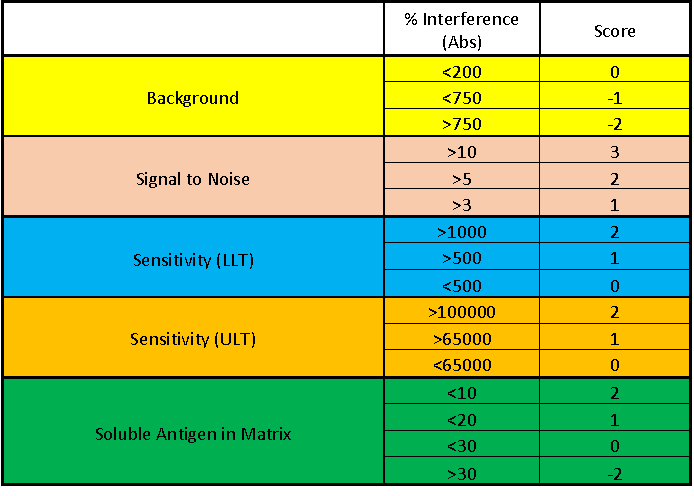
\includegraphics{graphics/ch3/Table_1.pdf}
\end{table} 
 
The example below shows calculation of the Anti-ID 6-Biotin & Anti-ID 6-Tag pairing assay to show how the scores are calculated. The Score fields are empty in the table below and will be filled based on each analytical parameter value.

\begin{table}[ht]
 \centering
 \caption{Excel table displaying example calculations for Anti-ID 6-Biotin + Anti-ID 6-Tag pairing results.}
 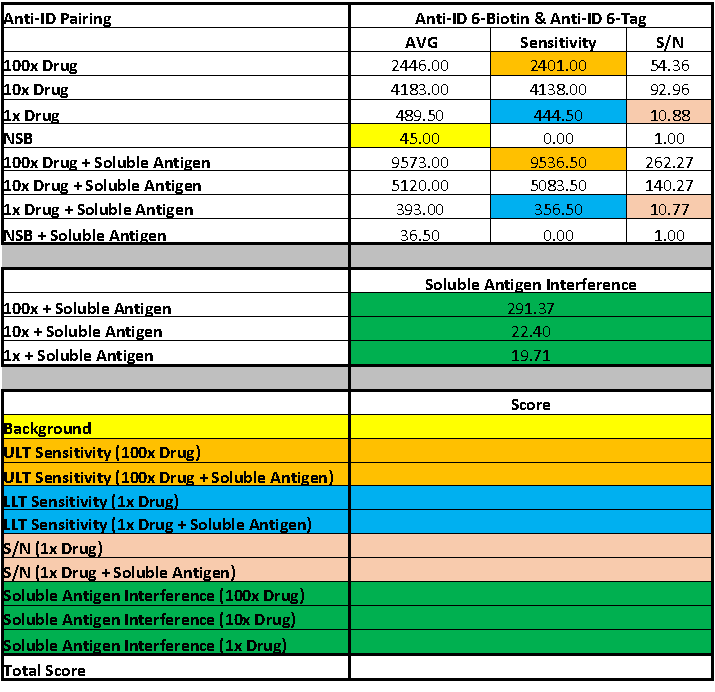
\includegraphics{graphics/ch3/Table_2.pdf}
\end{table} 

We will discuss each of the analytical metric based on the human-defined thresholds to calculate the scores.
\subsection*{Background Calculation:}
The data being scored is highlighted yellow in the table below.  As the background value above is 45, it is$ <$200 and was given a score of “0” shown below.

If the background is below a human-defined absolute value of 200 then it would receive a score of 0; for value between 200 and $<$750, the score is -1 and for value $geq$750, the score of -2.  The negative numbers were chosen for higher backgrounds as high background negatively impacts the assay and this concept was captured by assigning a negative score.  The ranges and score values were decided by human analysts.

For the background score, the higher the background the more negatively this impacted the PK assay and therefore it was assigned a negative score.  It however did not need to be assigned a negative score – it was only given this as it was determined to call out the negative impact on the assay.  The other “positive” scores were given with higher numbers to assign low interference and/or characteristics that would result in a robust sensitive assay.  

\vspace{-1cm}
\begin{table}[ht]
 \centering
 \caption{Excel table displaying background scoring for Anti-ID 6-Biotin + Anti-ID 6-Tag pairing results.}
 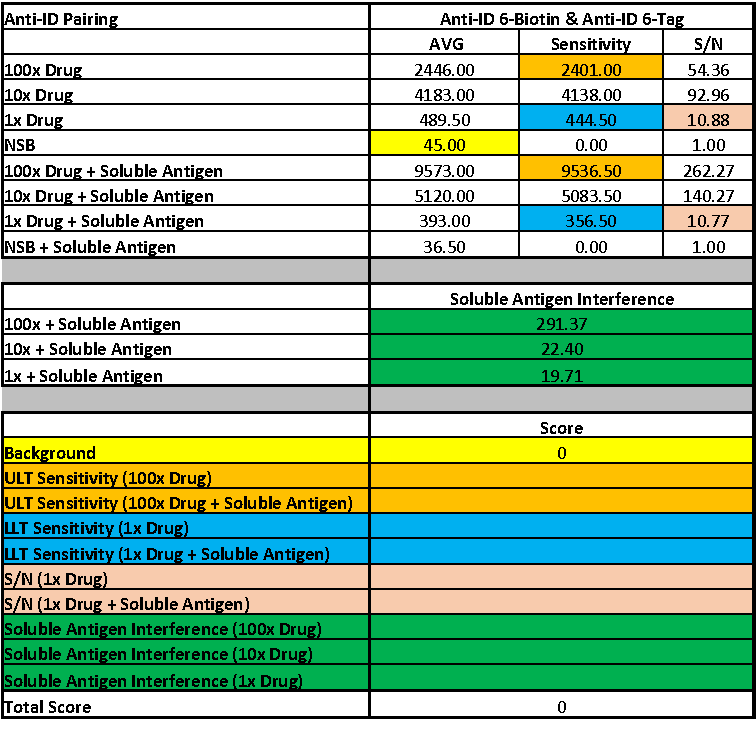
\includegraphics{graphics/ch3/Table_3.pdf}
\end{table} 

\subsection*{Sensitivity (Upper Limit Tested (ULT)) Calculation:}
The data being scored is highlighted orange in the table below.  As the ULT Sensitivity (1x Drug) was 2401.0, it is $<$65000 and was given a score of “0”, for ULT Sensitivity (1x Drug + Soluble antigen) was 9536.5, it is $<$65000 and was also given a score of “0”.

There are two values to be captured for this score +/- soluble antigen.  If the absolute value of the 1x Drug measurement is below 65000 then it would receive a score of 0; between 65000 to $<$100000, it was given a score of 1, and value $\geq$100000, a score of 2 was given.  The positive numbers were chosen for sensitivity (ULT) as the higher the numbers the more robust the assay and this concept captured by assigning a positive score.  The ranges and score values were decided by human analysts.

\begin{table}[ht]
 \centering
 \caption{Excel table displaying sensitivity (ULT) scoring for Anti-ID 6-Biotin + Anti-ID 6-Tag pairing results.}
 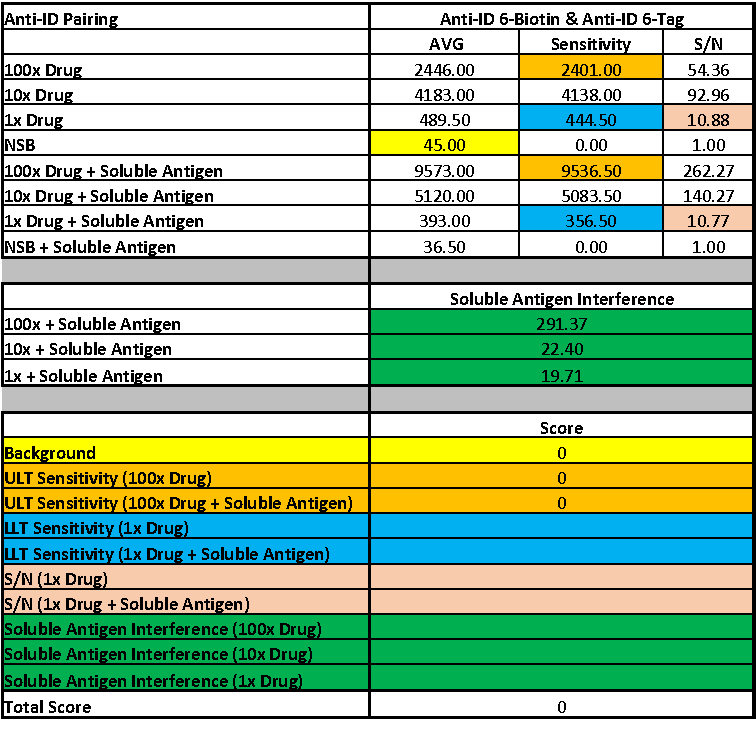
\includegraphics{graphics/ch3/Table_4.pdf}
\end{table} 

\subsection*{Sensitivity (Lower Limit Tested (LLT)) Calculation:}
The data being scored is highlighted blue in the table below.  As the LLT Sensitivity (1x Drug) was 444.5, it is $<$500 and would give a score of “0”, and the LLT Sensitivity (1x Drug + Soluble antigen) was 356.5, it is $<$500 and would also give a score of “0”.

There are two values to be captured for this score +/- soluble antigen.  If the absolute value of the 1x Drug measurement is below 500 then it would receive a score of 0; between 500 to $<$1000, it would receive a score of 1, and $\geq$1000 it would receive a score of 2.  The positive numbers were chosen for sensitivity (LLT) as the higher the numbers the more robust the assay and this concept was captured by assigning a positive score.  The ranges and score values were decided by human analysts.

\begin{table}[H]
 \centering
 \caption{Excel table displaying sensitivity (LLT) scoring for Anti-ID 6-Biotin + Anti-ID 6-Tag pairing results.}
 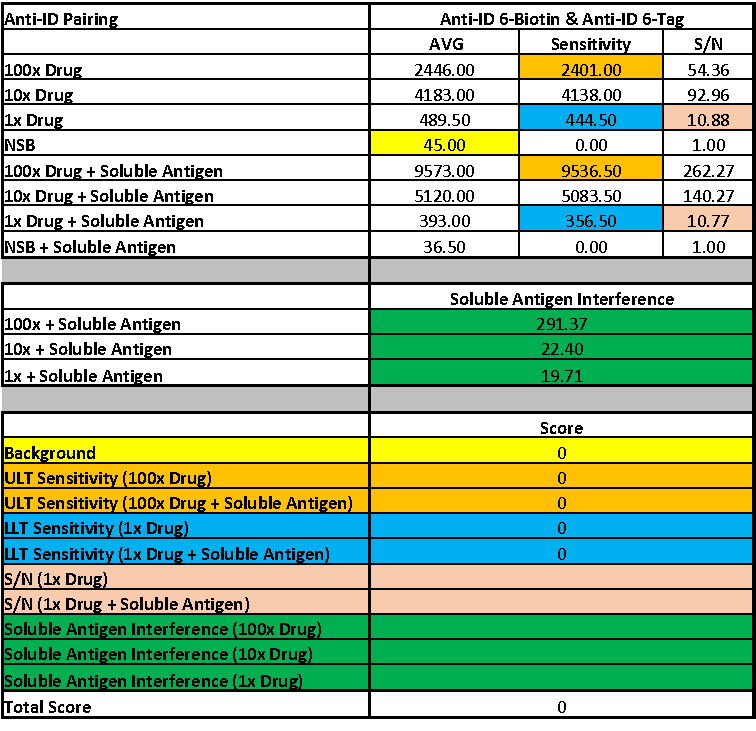
\includegraphics{graphics/ch3/Table_5.pdf}
\end{table} 

\subsection*{Signal to Noise (S/N) Calculation:}
The data being scored is highlighted peach color in the table below.  As the S/N (1x Drug) was 10.88 – it is $>$10 and would give a score of “3”; and the S/N (1x Drug + Soluble antigen) was 10.77 it is $>$10 and would give a score of “3”.

There are two values to be captured for this score +/- soluble antigen. If the absolute value of the 1x Drug measurement/divided by the background is $\leq$3 then it would receive a score of 0; for values $>$3 and $\leq$5, a score of 1; values $>$5 and $\leq$10, it would receive a score of 2 and for values $>$10 then it would receive a score of 3.  The positive numbers were chosen for S/N as the higher the numbers the greater the signal is away from background indicating a strong signal that will yield a robust the assay and this concept was captured by assigning a positive score.  The ranges and score values were decided by human analysts.

\begin{table}[ht]
 \centering
 \caption{Excel table displaying signal to noise scoring for Anti-ID 6-Biotin + Anti-ID 6-Tag pairing results.}
 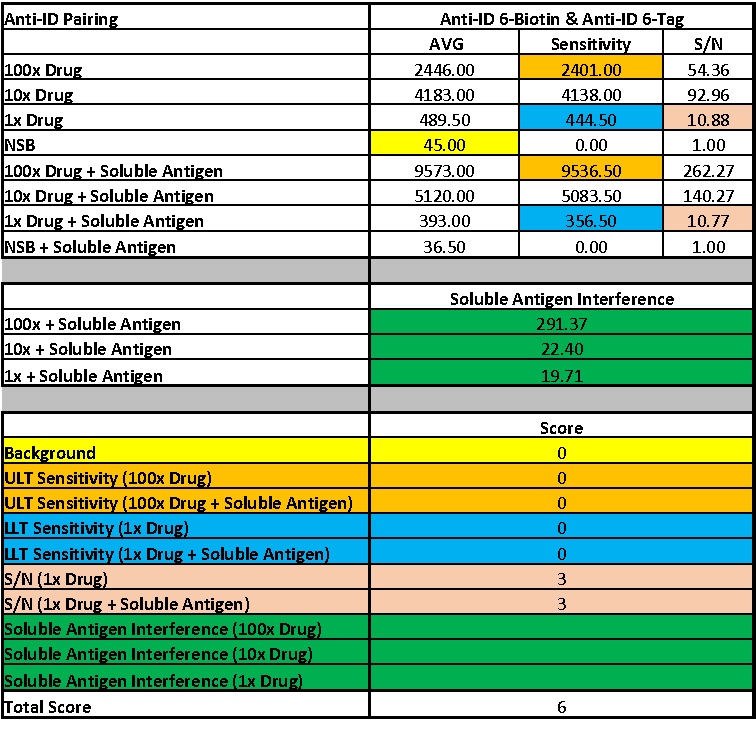
\includegraphics{graphics/ch3/Table_6.pdf}
\end{table} 

\subsection*{Soluble Antigen Interference Calculation:}

\\The data being scored is highlighted green in the table below.  For 100x drug soluble antigen interference value of 291.37, the score is -2, for 10x drug soluble antigen interference value of 22.40, the score is 0, for 1x drug soluble antigen interference value of 19.71, the score is 1.

There are three values to be captured for this score soluble antigen with the 3 different concentrations of drug used.  As an example,
\\
\\
\hspace*{.5in}100x Drug Soluble Antigen Interference = absolute value of
\\
\\
\hspace*{.5in}100*[(100x Drug Average–(100x Drug & Soluble Antigen Average)/(100x Drug Average]
\\
\\
\indent If the absolute value of the soluble antigen interference for X Drug measurement is $<$10 then score is 2; value $\leq$10 and $<$20 will get a score of 1, value $\geq$20 and $<$30 then the score is 0, value $\geq$30 then the score is -2.  The decreasing positive numbers were chosen for soluble antigen interference as the higher the numbers the greater the negative impact on the assay and this concept was captured by assigning decreasing positive scores.  The ranges and score values were decided upon by a collection of analysts.

Adding all the scores lead to the total score of 5, as shown in the table below.

\begin{table}[ht]
 \centering
 \caption{Excel table displaying soluble antigen interference scoring and total scoring for Anti-ID 6-Biotin + Anti-ID 6-Tag pairing results.}
 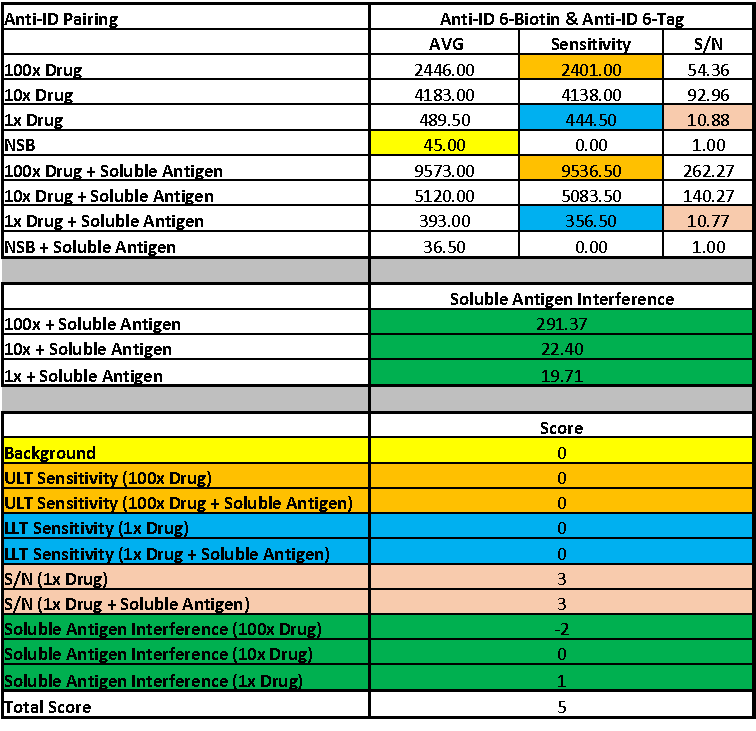
\includegraphics{graphics/ch3/Table_7.pdf}
\end{table} 

\subsection{Scoring Tool}
Initial reagent screening using the ECL assay format focused on interference from the matrix and soluble antigen.  The screening of labeled pairs using different assay formats used a more complex scoring function.  The parameters assessed in this scoring function included background signal, signal to noise, sensitivity, dynamic range, and soluble antigen interference.  These parameters were assessed using 6 different assay formats and at two different anti-ID concentrations. A total score was calculated based on the listed criteria, where analytical parameters were assigned scores.  Parameters with high values, such as background, were given negative scores and positive scores for low values.  The negative numbers were chosen for higher backgrounds as high background negatively impacts the assay and this concept was attempted to be captured by assigning a negative score.  The positive numbers were chosen for sensitivity (ULT, LLT) as the higher the numbers the more robust the assay. The positive numbers were chosen for signal to noise (S/N) as the higher the numbers the greater the signal is away from background indicating a strong signal that will yield a robust assay. The decreasing positive numbers were chosen for soluble antigen interference as the higher the numbers the greater the negative impact on the assay and this concept was attempted to be captured by assigning decreasing positive scores. The ranges and score values were decided by human analysts. However, the use of negative values during scoring was omitted when using data dependent scoring methods.  The initial use of negative values was chosen for ease of interpretability for identifying negative impacts on the assays.

The screening of multiple reagents and assay formats resulted in many assay plates with a large volume of data to be processed to enable the selection of the optimal reagents for the PK assay.  The scoring function was designed to enable the assay developer to weight parameters differently based on assay requirements.  Manually processing this data using a spreadsheet is time-consuming and potentially can introduce errors.  In order to streamline this process, the scoring tool was programmed in Python with a graphical user interface (GUI) to accelerate data processing and provide consistency in using the tool (Supplementary Figures S1-3). 

\begin{figure}[ht]
 \centering
 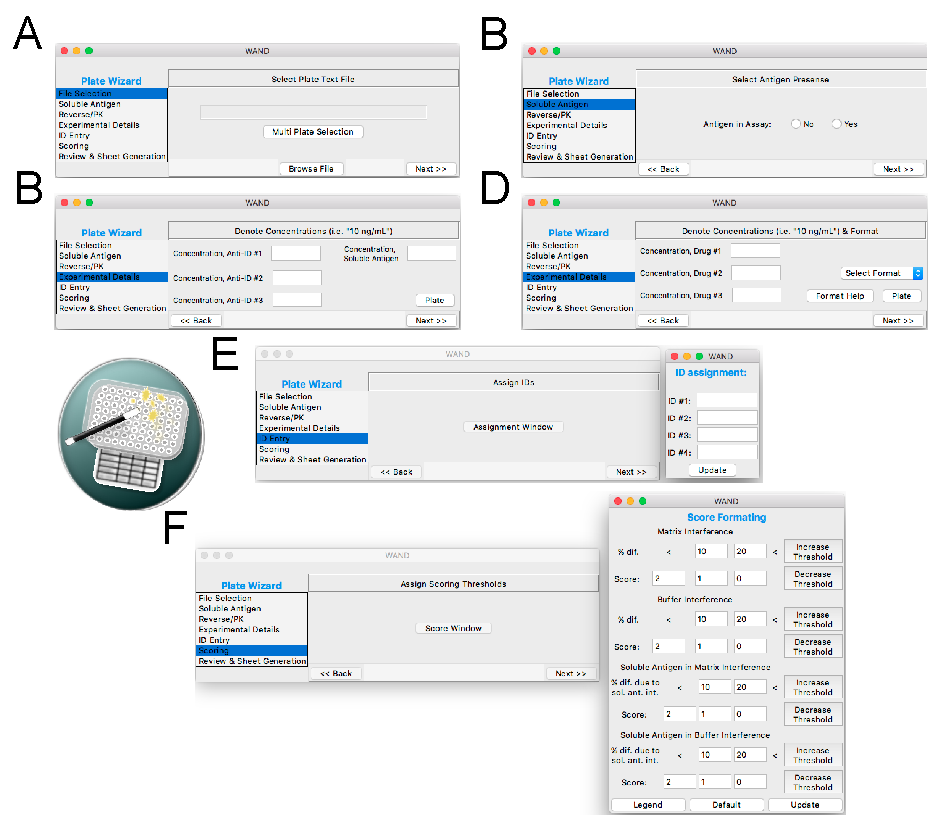
\includegraphics{graphics/ch3/Figure_S1.pdf}
 \caption{WAND: Workflow Automation for Nested Decision is a software tool with graphical user interface to automate experiment set-up and data analysis by incorporating information on several assay formats, detailed error handling for specific formats and automated data analysis to minimize human error. The user specifies different assay parameters, conditions, and scoring weights, generating comprehensive reports as excel sheets for further analysis. (A) The file selection panel allows WAND to access and process plate reader files. (B) The antigen selection and screening type panels allow the user to specify the appropriate experimental descriptors for a given plate reader file.  (C&D) The experimental details, and subsequent panels, are displayed such that prior specifications dictate the inputs available that ensure proper descriptor entry.  (E) ID entry is performed in a separate window which allows users to input the appropriate name of reagents.  (F) Dynamic scoring entry allows for users to modify the interpretation of plate reader files such that desired analytical values are given higher pertinence post analysis.}
 \end{figure}
 
\begin{figure}[ht]
 \centering
 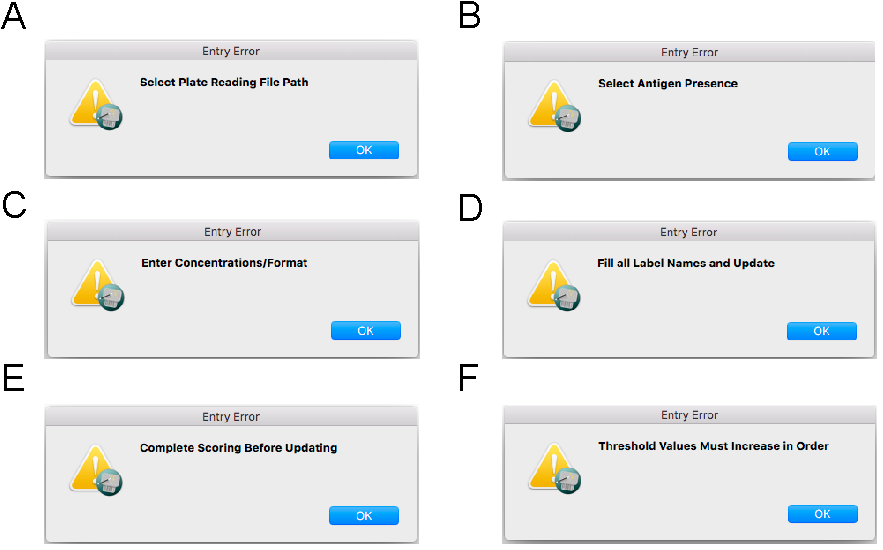
\includegraphics{graphics/ch3/Figure_S2.pdf}
 \caption{Showing error handling in WAND to ensure all information needed to produce a complete data analysis report is provided by the user.  Error statements are prompted by premature toggling of the next interface display when: (A) no plate reader file is uploaded, (B) no selection of antigen presence in a plate assay and similarly if a generic or PK screen was run, (C) descriptive experimental details such as drug concentration or PK format are omitted when required, (D) absent reagent label descriptors, (E) absent values when entry boxes are present in the scoring window, and (F) the entry of non-increasing numeric values for the thresholds of a given analytical scoring metric.}
 \end{figure}

\begin{figure}[ht]
 \centering
 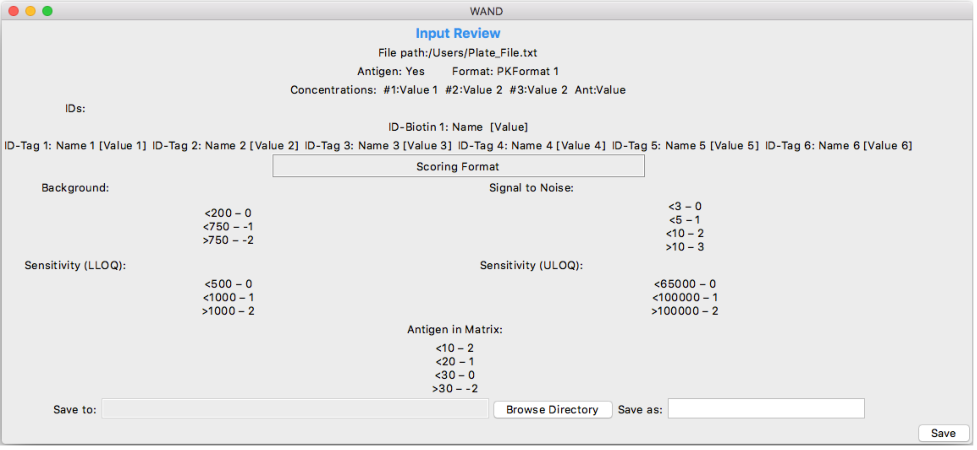
\includegraphics{graphics/ch3/Figure_S3.pdf}
 \caption{Example of a review screen prompted by WAND prior to generation of an analysis report sheet.  All user inputs are captured and displayed to allow users to ensure the correct information has been provided prior to designating the location and name of the report to be generated.}
 \end{figure}

\subsection{Data Dependent Scoring}
The scoring functions used for ranking ECL-based anti-ID screening and PK assay formats along with anti-ID pairing screens were done in a data-dependent manner using Gaussian mixture models (GMMs).  Instead of using predetermined human-identified thresholds, GMMs fits a number (\emph{K}) of weighted Gaussian distributions called mixture components to the data.  By fitting the values of assay conditions evaluated by scoring functions, the GMM pipeline clusters and classifies data-points (\emph{x}) into a class (\emph{c}) corresponding to a mixture component.  The data-points are classified by treating their maximal probability under the weighted Gaussian distributions as their ‘class label’ (y\textsubscript{\emph{l}}) as given in eq. 3.1. 

\begin{equation}
y_l:=\argmax_ip(c_i\vert x),\,c_i\in \{0…K\}
\end{equation}
The GMM pipeline was developed such that the number of Gaussian distributions was selected by fitting GMMs with the number of Gaussians ranging from four to ten and selecting the model with the lowest resulting Akaike information criterion.  Absolute values of data-points were first min-max normalized prior to evaluation using the GMM based data dependent scoring pipeline.  The GMM based data dependent scoring pipeline was implemented by fitting GMMs to both individual parameters and the full set of parameters simultaneously.  For cases where lower values are desired for parameters used to evaluate PK assays, the absolute values of data-points were made negative prior to normalization when evaluating all parameters simultaneously.  Scores for ranking were assigned to clustered data points by assigning increasing integer values, starting from zero.  The Euclidean norm was used to measure cluster means from a vector comprised of elements all equal to zero or all equal to one for ECL-based anti-ID screening and PK assays respectively, when evaluating all parameters simultaneously.  Clusters were then assigned their rank order, starting from zero, in order of decreeing Euclidean distance measures.  When evaluating individual parameters, cluster means would have their measures calculated from either zero or one vectors depending on if lower or greater parameter values were respectively desired.  

Covariance regularization of the mixture models was applied when evaluating individual parameters such that elements of the covariance matrix off the diagonal were weighted to zero.  Otherwise, the covariance matrixes were unregulated when evaluating all parameters simultaneously.  GMMs were implemented using the Scikit-learn (Version 1.0.2) Python library with all parameters, excluding the number of components and covariance regularization types, left as default values.  Results were visualized using Uniform Manifold Approximation and Projection (UMAP) for cases where all parameters were evaluated.  UMAPs were generated using the umap-learn (Version 0.5.3) Python package.  For the generic indirect ELISA screening studies UMAP parameters were defined as: \emph{‘n{\_}components’} set to 2 , \emph{‘n{\_}neighbors’} set to 15, and \emph{‘min{\_}dist’} set to 0.25.  For PK studies UMAP parameters were defined as: \emph{‘n{\_}components’} set to 2 , \emph{‘n{\_}neighbors’} set to 50, and \emph{‘min{\_}dist’} set to 0.25.  Both uses of UMAP used a Euclidean metric. Cumulative scores were summed from min-max normalized GMM produced scorings, with normalization being applied to the scores of each experimental trial with varied concentrations of antigen or anti-IDs.  All code for GMM and UMAP studies was run in Python 3.7.11, and is available with plots on Github at \emph{https://github.com/chopralab/Bioanalytical\textunderscore Assay\textunderscore Manuscript\textunderscore Repo/tree/main/GMMs}.


\section{Results}
\subsection{Generation of Anti-IDs and Initial Selection}
Anti-idiotypic antibodies were generated using the Fab fragment of a proprietary therapeutic antibody.  Ten mice from 2 different strains were immunized 3 times and serum was collected.  The antibody titer for each mouse was determined using an ELISA assay with the therapeutic Fab region used as the capture and a goat anti-mouse IgG-HRP was used for detection.  Two mice with the highest titers were euthanized for generation of hybridomas with their lymphocytes from spleens and the myeloma fusion partner.  This resulted in 18 clones with specific binding to the mAb from the primary screening of the anti-ID antibodies (Table S1).  This panel of anti-IDs were high affinity antibodies with most KD values less than 100 nM (Table S2).    The epitope binning data indicated that the 18 anti-IDs all bind to closely related epitopes and are in the same epitope bin with the response percentages $<$10\% (Table S3).  The resultant 18 clones were chosen for further screening to determine the optimal anti-IDs to bind to the mAb in the presence of soluble antigen.

\begin{figure}[ht]
 \centering
 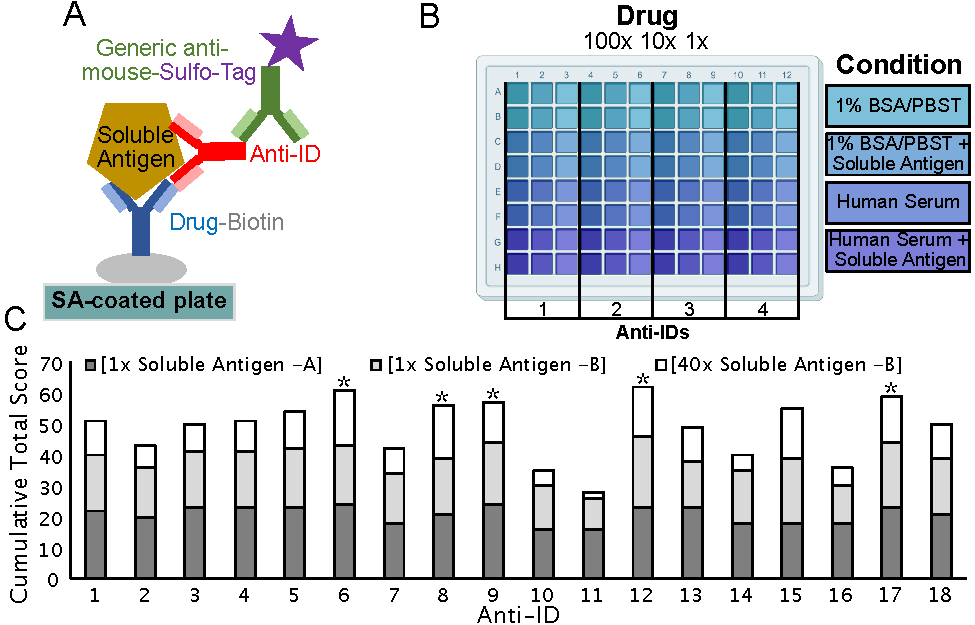
\includegraphics{graphics/ch3/Figure_1.pdf}
 \caption{Generic indirect ELISA initial screen of anti-IDs in the presence of matrix and soluble antigen. A) Schematic diagram of generic indirect ELISA with soluble antigen. B) Representative plate layout for generic ELISA screen.  Four anti-IDs across 2 orders of magnitude of concentration were screened per plate +/- human serum and/or soluble antigen.  C) Scoring matrix used to rank order anti-IDs based upon impact of matrix and soluble antigen interference.  D) Cumulative total scores for anti-IDs in the presence of 1x or 40x soluble antigen.  (*) indicate anti-IDs selected for labeling.}
 \end{figure}

Traditional methods for functional screening of anti-IDs involved labeling each anti-ID for capture and detection.  For 18 different anti-IDs this is a laborious process resulting in a large number of labeled reagent enumeration to screen every potential pairing.  To this end, 324 different combinations would need to be tested per assay format, at a single concentration, if a traditional approach was used.  Therefore, an indirect format (Figure 1A,B) was used to perform an initial screen of anti-IDs to examine the effects of matrix (pooled human serum) and soluble antigen interference on the ability of the anti-IDs to bind to the therapeutic antibody.  A standardized plate map was also selected to allow for development of automation procedure and for the future use of this workflow in screening anti-IDs in other projects.  In addition, a scoring system was established to rank order the anti-IDs based on the effect of 1) soluble antigen interference in buffer, 2) matrix interference (blank serum), 3) soluble antigen in matrix versus buffer, and 4) soluble antigen in matrix versus blank matrix (Figure 1C).  This was performed at three levels of each anti-ID (1x, 10x, 100x) in the presence of soluble antigen that was calculated to be at least 10x greater than the lowest expected levels of soluble antigen in patients.  Additionally, this format was tested in the presence of 40x of the soluble antigen for super saturating conditions of soluble antigen.  The composite scores from each experiment were tabulated and are shown in Figure 1D. Complete data and scoring are in Supplementary Tables 4-6.  The top five anti-IDs (6, 8, 9, 12, 17) with the highest composite score and the least interference from matrix and/or soluble antigen were then selected for progression to a more rigorous labeled-anti-ID sandwich assay format. 

\begin{figure}[ht]
 \centering
 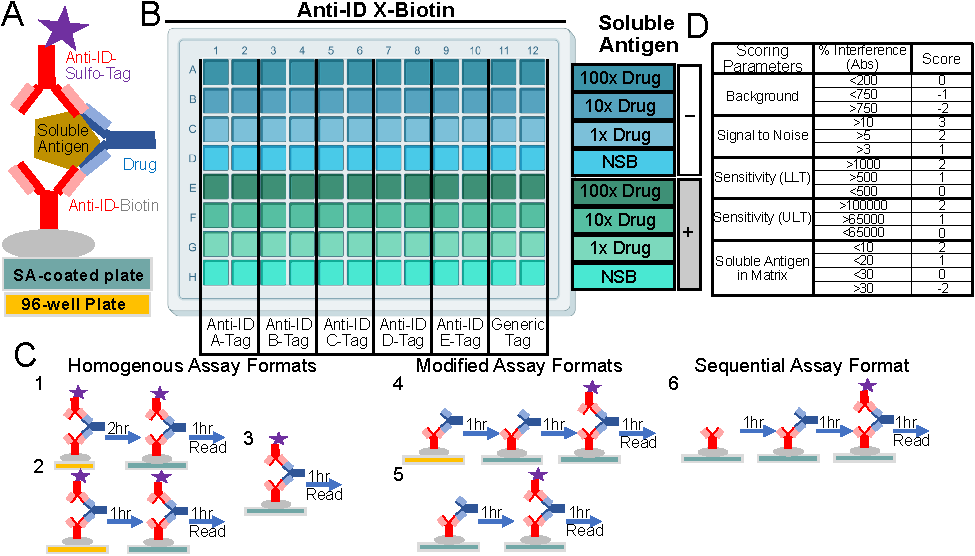
\includegraphics{graphics/ch3/Figure_2.pdf}
 \caption{Labeled anti-ID pairings and sandwich PK assay format screening approach.  A) Schematic diagram for sandwich anti-ID ELISA screening.  B) Representative plate map for labeled anti-ID screen.  Six Sulfo-TAG-anti-IDs were used per plate with a single biotinylated-anti-ID to measure the concentration of therapeutic $\geq$2 orders of magnitude +/- soluble antigen.  The non-specific binding (NSB) +/- soluble antigen was also measured.  C) PK assay formats screened.  Six PK assay formats were screened: three homogenous formats, two modified assay formats, and one sequential assay format. D) Scoring matrix for rank ordering of anti-ID pairings with analytical parameters using absolute interference.}
 \end{figure}


The five selected anti-IDs (6, 8, 9, 12, 17) were labeled with biotin and Sulfo-tag and used as both capture and detection reagent in the next screening step (Figure 2A).  These labeled reagents were used to determine the best pairing for a PK assay resulting in 25 different possible pairing combinations.  Additionally, a generic mouse anti-human IgG4 was used as a detection reaction in combination with the 5 different capture reagents for a total of 30 pairing combinations.  A standardized plate map was again utilized to enable use of automated liquid handlers and the automated scoring tool (Figure 2B).  The anti-ID screening for PK assay development has historically been done on a ‘fit-for-purpose approach’ wherein the anti-IDs are typically screened in a pre-defined assay format at a single concentration [17]. Once the reagent pair is identified by the pre-defined assay format, other assay formats are tested to further optimize the performance of the assay. However, a limitation exists, in that the best reagent pair selected by the pre-defined assay format is not necessarily the best pair of reagents for other assay conditions. Given the interdependence of reagents combination, concentration and assay formats, a more comprehensive approach was developed with 30 anti-ID pairings that were tested with two different concentrations (0.25 µg/mL and 1.0 µg/mL) in six different PK assay formats (Figure 2C).  These pairings of anti-IDs were screened across $\geq$2 orders of magnitude of the mAb +/- soluble antigen.  

\begin{figure}[H]
 \centering
 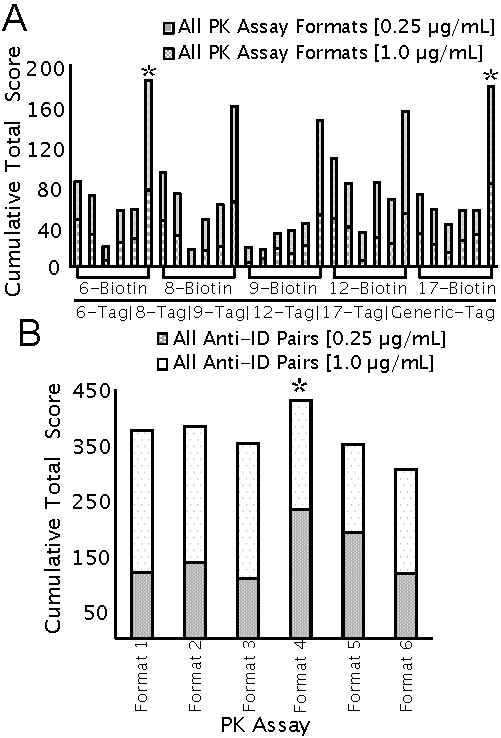
\includegraphics{graphics/ch3/Figure_3.pdf}
 \caption{Labeled anti-ID pairings and sandwich PK assay format screening results. A) Cumulative total score of two concentrations of anti-ID pairings across all PK assay formats.  Scores were established for each anti-ID pairing/PK assay format per concentration.  The scores of all six PK assay formats per anti-ID pairing were tabulated.  The top two pairings across all PK assay formats are indicated by (*).  B) Cumulative total score of PK assay formats across all anti-ID pairings.  The scores of all anti-ID pairings per PK assay format were tabulated.  The top PK assay format is indicated by (*).}
 \end{figure}

A second scoring system was developed to determine both the best pairing and optimal PK assay format.  The parameters measured and scored include: 1) background signal, 2) signal to noise, 3) sensitivity LLT (lower therapeutic concentration counts), 4) sensitivity ULT (upper therapeutic concentration counts), and 5) soluble antigen in matrix (Figure 2D).  Parameters 1 to 4 were assessed in the presence and absence of soluble antigen.  The cumulative scores for both concentrations of anti-IDs across all PK assay formats tested are displayed in Figure 3A.  The generic-tag detection reagent was the best detection reagent regardless of the anti-ID capture or concentration as the top five scores all had the generic-tag for detection (Figure 3A; Supplementary Table 4, 5).  Further, the anti-ID #6 had the greatest cumulative score across all PK assay formats tested with anti-ID 17 selected as the back-up with the second top score.  The pairing of anti-ID #6-Biotin/Generic-Tag had the maximal score, 20, in both concentrations tested, while the pairing of anti-ID #17-Biotin/Generic-Tag had the maximal score at 0.25 g/mL and a score of 18 at 1.0 µg/mL due to soluble antigen interference at 10x drug (Supplementary Table 4, 5).  These anti-IDs were both selected to generate large-scale recombinant proteins for future use in the development and validation of the clinical PK assay.  Assay format 4 had the greatest cumulative score for all anti-IDs across both concentrations tested (Figure 3B; Supplementary Table 4, 5) and was selected as the optimal PK assay format.  

\begin{figure}[H]
 \centering
 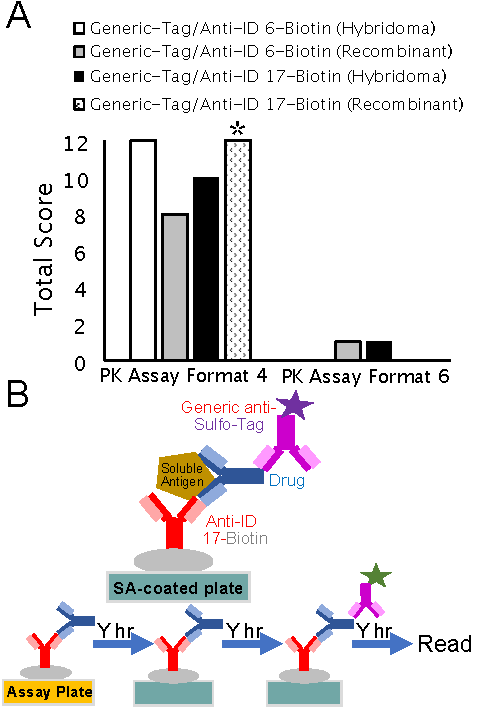
\includegraphics{graphics/ch3/Figure_4.pdf}
 \caption{Final anti-ID pairing and PK assay format selection.  A) Recombinant anti-ID pairings were compared to original hybridoma pairings in two different PK assay formats.  Scores were calculated based upon previous criteria listed in Figure 2D.  The total score of for each pairing/format was tabulated.  The final recombinant pairing selected is indicated by (*).  B) Schematic of final anti-ID pairing and PK assay format that were selected.}
 \end{figure}


Large-scale recombinant proteins for anti-ID #6 and #17 were generated and these pairings were compared with the original hybridoma reagent pairings in PK assay formats 4 and 6 to confirm the selection of optimal PK assay format and anti-ID pairing (Figure 4A; Supplementary Table 6).  PK assay format 4 yielded higher scores relative to assay format 6 indicating this to be the optimal PK assay format for these anti-ID pairings.  There was a decrease in sensitivity and signal to noise scores that resulted in a decreased total score for the anti-ID 6-Biotin/Generic-Tag recombinant pairing compared to the hybridoma pairing.  However, there was an increase in signal to noise score in the anti-ID #17-Biotin/Generic-Tag recombinant compared to the hybridoma (Figure 4A).  This increased total score resulted in the selection of anti-ID #17-Biotin/Generic-SulfoTag recombinant pairing in PK assay format 4 as the final PK assay (Figure 4B). 
\subsection{Scoring Tool and Graphical User Interface}
Data handling and analysis is a tedious task during an execution of automated assays formats. The scoring metrics for generic and PK assay formats was compiled with Workflow Automation for Nested Decisions (WAND) to facilitate the rapid analysis of data from several experiments to make decisions (Figure S1). Further, detailed error handling for specific formats was implemented to minimize human error during experimental set-up, parameter selection and interpretation (Figure S2). The user specifies different assay parameters, conditions and scoring weights in a stepwise manner to generate comprehensive reports (Figure S3) for further analysis. The modularity of the GUI makes it easy to go beyond the six specified PK assay formats and makes WAND an ideal choice to develop robust automated PK assay workflows.

\subsection{Gaussian Mixture Model Based Scoring}

\begin{figure}[H]
 \centering
 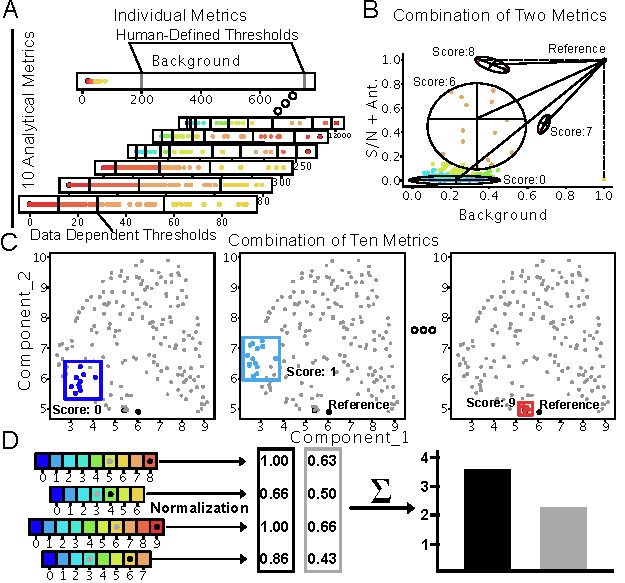
\includegraphics{graphics/ch3/Figure_5.pdf}
 \caption{Schematic of data dependent scoring.  Showing representative data for PK assays (1µg/mL) A) Data from individual metrics were clustered using GMMs, resulting in new thresholds (black) which further differentiate interference distributions compared to human-defined thresholds (grey).  B) Extension of the GMM scoring approach where data from two metrics are clustered simultaneously.  Clusters are ranked by their mean distance from a point defined by the best values of each individual analytical parameter.  C) Extension of the GMM scoring approach by incorporating all 10 analytical parameter associated with PK assays.  Clustering is done in 10-Dimensional space, and displayed as a 2-Dimensional UMAP, with selected clusters displaying their respective coloring and scores. Reference indicates the origin or the best possible score in higher dimensions which is used for scoring clusters.  D). Schematic displaying the scoring to assay ranking pipeline, where scores derived from GMM clusters are normalized and followed by summation.}
 \end{figure}

The scoring systems previously described were replicated in a data dependent manner by use of GMMs.  Evaluation of parameters was done both by fitting GMMs to each parameter individually and by fitting a single GMM using data-points representing vectors comprised from normalized values from each parameter (Figure 5).  The data dependent scoring approach replicated selections derived from cumulative scores with high overlap.  Using the approach of fitting GMMs to each parameter individually, two of the selected anti-IDs from ECL-based screening again yielded cumulative scores within the top five (Figure S4-7) and fully replicated the selections for anti-ID pairings and PK assay format (Figure S8-9).  When using a single GMM to evaluate all parameters simultaneously, the perfect overlap in PK assay results was maintained, while identifying an additional anti-ID that was selected using human-defined thresholds for evaluating ECL-based screenings.  

\section{Discussion}
Ligand binding assays (LBAs) have been widely used to quantify the amount of biological drug molecules in pharmacokinetic studies.  The reagent screening and assay development of LBAs to measure PK have traditionally used a semi-empirical approach.  However, the increased usage and development of therapeutic antibodies presents an opportunity to develop and use a systemic approach to increase efficiency, quality, and robustness of the LBA PK assay.  For some therapeutic antibodies, the presence of a circulating soluble target could interfere with the PK assay performance and requires consideration to ensure total drug levels can be measured, that includes both free and target-bound drug.  Identification of reagents with a high binding affinity specifically for the mAb regardless of presence of soluble target and a low matrix interference are key qualities for the optimal reagent.  However, the most robust PK assay cannot be developed with such reagents if the optimal PK format for these reagents has also not been selected.  Therefore, screening and selection of critical reagents concurrently with the determination of the most robust assay format are key components in developing a robust PK assay capable of measuring free and bound mAb levels in serum.    
  
Anti-IDs were generated through creation of hybridomas from immunizations of mice with the Fab fragment of the therapeutic mAb.  Multiple characteristics of the anti-IDs including the binding kinetics, affinities for the mAb and epitope binning were determined to attempt to triage the number of Anti-IDs to be screened.  The results of the binding kinetics and affinities showed similar characteristics for all anti-IDs generated in the present study, and all of these anti-IDs were found to be in the same epitope bin.   These results required all 18 anti-IDs to move forward to be screened to determine the optimal reagents for the PK assay.  However, these results did not account for the effects of matrix and/or soluble antigen interference on the ability of the anti-IDs to bind to the mAb.  In addition, hybridomas often lead to a large number of clones and it is inefficient and costly to label and screen all clones.  Therefore, a two-step strategy was developed to identify optimal reagents and assay format to differentiate and select anti-IDs using an ECL screening assay and then a labeled anti-ID sandwich ECL screening assay with a GUI to do multiple scoring parameters analysis.  This strategy was successful in identifying the most robust PK assay format with the optimal reagents for a mAb.    

The first phase of the strategy involved using a generic screen of the anti-IDs with a biotinylated mAb as a capture and an anti-mouse IgG-HRP as a detector (Figure 1A-B).  This initial screen allowed for determination of both the effect of matrix and soluble target interference on the ability of the anti-IDs to bind to the mAb.  A scoring system was used to rank-order the anti-IDs that assigned a numerical value to four different parameters based upon the effects of matrix and soluble antigen interference (Figure 1C, D; Supplementary Tables 1,2,3).  The use of this scoring system allowed for identification of anti-IDs that had the lowest cross-reactivity to human serum and interference from soluble antigen.  Identifying the anti-IDs with the top scores decreased the number of pairs of anti-IDs to use in a labeled screen and allowed for a more targeted investigation into the optimal anti-IDs and PK assay format.  The top five performing anti-ID’s based on their scores and a generic detection reagent were chosen to move to the second stage of screening.

Following the selection of anti-IDs for the second phase, the anti-IDs were both biotinylated and Sulfo-tagged to be used in a pairwise sandwich ECL assay with the therapeutic mAb.  This screening was done at three concentrations of mAb across at least 2 orders of magnitude in the presence and absence of the soluble target.  In addition, six different PK assay formats and two concentrations of anti-IDs were used to simultaneously identify the most robust PK assay format and optimal reagent combination and concentration.  A second scoring system measuring ten different parameters was used to determine the optimal anti-ID pairing and PK assay format (Figure 2C, D, Figure 3A, B; Supplementary Tables 4,5).  The ten parameters include, 1) background signal, 2) and 3) signal to noise with and without soluble ligand, 4) and 5) upper level of quantitation with and without soluble ligand, 6) and 7) lower level of quantitation with and without soluble ligand, and 8), 9) and 10) soluble ligand interference at three different drug levels. This multifactorial scoring system identified the top two performing pairs of ant-IDs in the PK assay format that would yield the most robust PK assay (Figure 3A and 3B).  These results were further confirmed by the results the recombinant anti-ID pairings (Figure 4A and 4B).  To enable this complex approach, all assay steps were automated on a liquid handling system to ensure consistency of the method given the range of pipetting steps required on each sample plate and the number of total plates created.

Anti-IDs clones #6 and #17 as capture and the generic a Sulfo-TAG-mouse anti-human IgG4 using assay format 4 were provided used to perform full assay optimization.  Recombinant versions of these clones were generated for further testing.  The modified assay format (Format 4, Figure 2C) of preincubation of the sample with the biotinylated capture reagent prior to transferring to the streptavidin MSD assay is not a typical format.  This approach was repeated and compared to the more traditional sequential format (Format 6, Figure 2C).   Soluble ligand that potentially could interfere with assay performance was used to test for interference.  Both the reagent from the hybridoma and the scaled up recombinant anti-ID confirmed that using the modified Format 4 provided better overall assay performance.  The recombinant version of the backup clone (Clone #17) provided better overall performance when compared to the recombinant version of Clone #6.  This reagent pair and assay format was taken into full assay validation to support the clinical development program.
The two-step screening strategy outlined herein provides a framework for efficient screening of anti-IDs and identification of the most robust PK assay format.  Using fixed plate maps in this approach allowed for the use of automation and development of the WAND scoring tool (Figure S1-3), which together provide an additional layer of uniformity and eliminates potential operational variability.  The scoring system that was developed was also designed to allow for changing of the weighting of the individual scores as needed.  This could occur if there is additional knowledge on the mAb or program indicating that a parameter has potentially more impact on the necessary PK results.  The scoring system for each parameter additionally can be expanded if there is a need to further differentiate the anti-IDs.  Combining fixed plate formats with easily interchangeable elements in this strategy allows for use of these tools in future anti-ID screenings and PK assay development.

\begin{figure}[H]
 \centering
 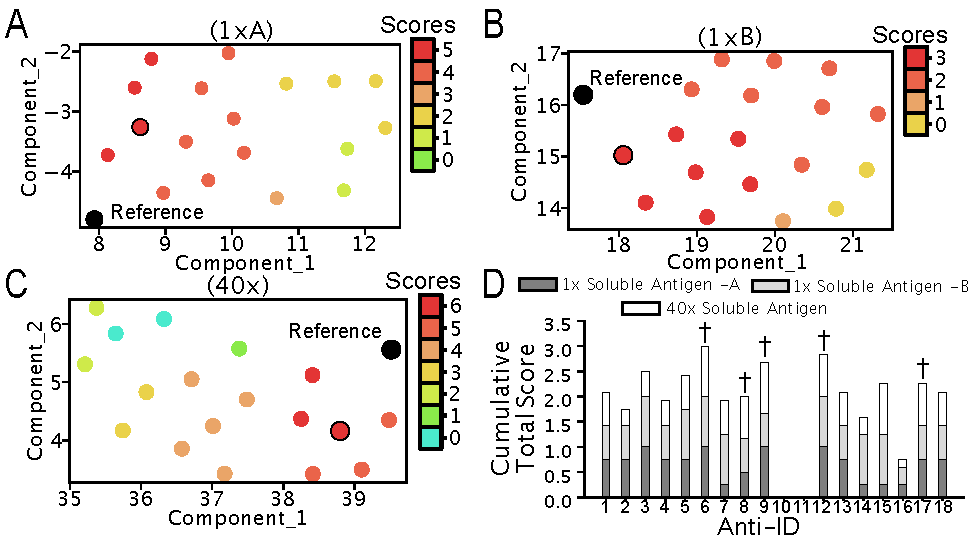
\includegraphics{graphics/ch3/Figure_6.pdf}
 \caption{GMM clustering and by combining all analytical parameters of generic indirect ELISA initial screen of anti-IDs in the presence of matrix and soluble antigens and cumulative scorings. UMAP embeddings of GMM clustered data-points comprised of the four analytical parameters at three concentrations of anti-IDs (total 12-Dimensions). Reference indicates the origin in 12-Dimensions with the best possible score.  A) Clustering of anti-IDs with 1x soluble antigen -A.  B) Clustering of anti-IDs with 1x soluble antigen -B.  C) Clustering of anti-IDs with 40x soluble antigen.  D) Cumulative total scores for anti-IDs in the presence of 1x or 40x soluble antigen.  (†) indicates anti-IDs selected for labeling by using human-defined thresholds for scoring.}
 \end{figure}

\begin{figure}[H]
 \centering
 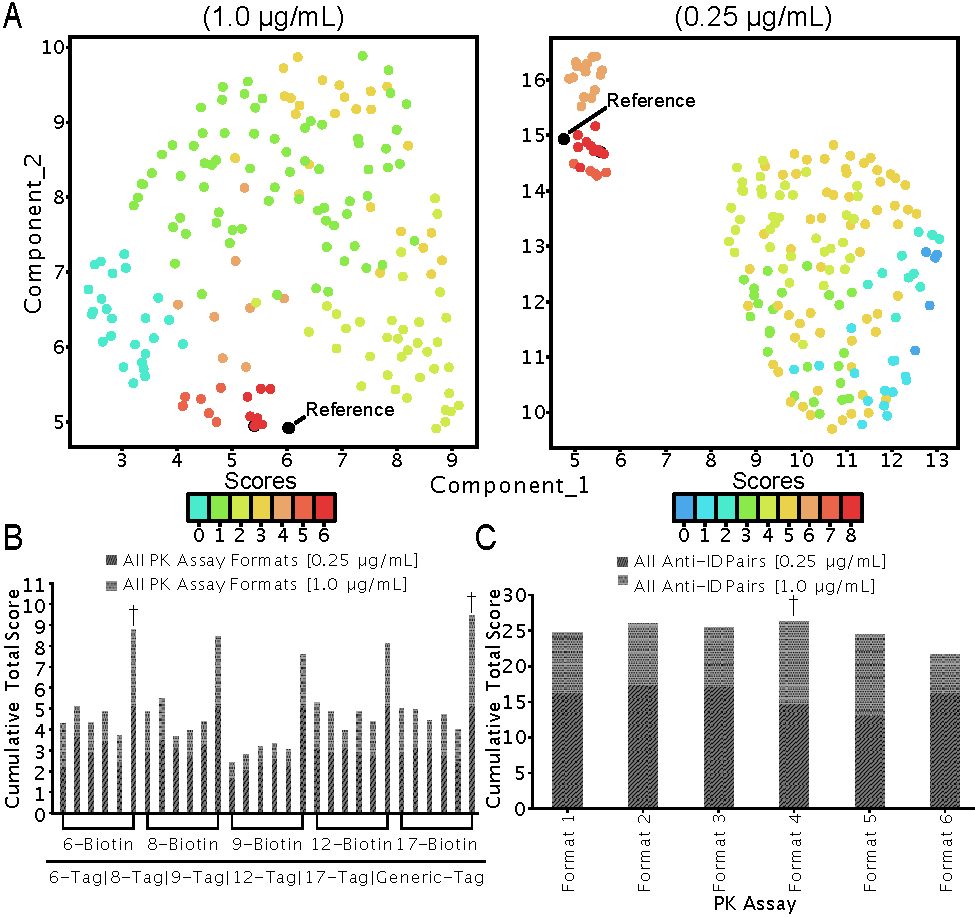
\includegraphics{graphics/ch3/Figure_7.pdf}
 \caption{GMM clustering and cumulative scoring of anti-ID pairings across several sandwich PK assay formats by combining all analytical parameters. UMAP embeddings of GMM clustered data-points comprised of the five analytical parameters, with ULT and LLT and signal to noise used in the presence and in absence of soluble antigen and soluble antigen interference at three separate drug concentrations (total 10-Dimensions). A) GMM clustering on a combination of all ten metrics at a concentration of 1 µg/mL and at a concentration of 0.25 µg/mL. Reference indicates the origin in 10-Dimensions with the best possible score. B) Cumulative total scores of anti-ID pairings across all formats.  Anti-ID pairings are plotted such that a biotinylated reagent and its six Sulfo-tag pairings are plotted sequentially, with the sequence of Sulfo-tag reagents repeating (see Figure 3A). C)  Cumulative total scores of PK assay formats across all anti-ID pairings.  (†) indicate the top anti-ID pairings and PK assay formats selected using human-defined thresholds for scoring.}
 \end{figure}

The data dependent scoring using GMMs broadly captured the robustness of the top assay conditions selected using human based thresholds for the analytical parameters used for scoring (Figure 6, 7, S7, S9).  While both evaluating parameters individually or in unison with GMMs fully replicated the selection of anti-ID pairings and formats for PK assays (Figure 9B-C, S9), the visualized results of individual parameter evaluation by GMMs show further differentiation of assay conditions compared to human based thresholds (Figure S5-7, S9).  Notable examples of the robustness of the GMM based scoring approach are displayed when fitting individual GMMs to PK assay screening results (Figure S9), such as where exceptional results regarding ULT sensitivity are furtherly reinforced.  The use of an automated data driven method for scoring assays removes a large component of human bias and eliminates errors introduced when scoring manually.  Future work on the scoring system aims to leverage automated data science driven approaches towards developing active learning methods. Such predictive machine learning algorithms will facilitate the generation of screening conditions to further expedite the selection and discovery of the optimal anti-IDs with minimum number of experiments.  We envision that developing automated frameworks will facilitate the development of ligand-based assays to enhance the discovery process without human bias.

\section{Conclusion}
An automated bioanalytical workflow for screening anti-IDs to determine the optimal pairing of reagents and PK assay format has been developed.  Fixed plate maps were employed for use with automation with an optimal and flexible scoring system to create a strategy that resulted in significant savings of time (days versus weeks) and resources to develop a novel and robust PK assay for a mAb.  With the increase of therapeutic antibodies as novel drugs, an automated assay and data dependent analysis strategy that allows for rapid identification of critical reagents and development of PK assay will become increasingly more important for supporting human clinical trials.  The proposed automated workflow and tools were successfully used to develop a bioanalytical assay for supporting a clinical program is being implemented for the continued support of antibody drugs. Automation based on learning from data will result in faster discovery and removal of human bias from data interpretation and candidate selection to develop new antibody drugs.

\section{Future Directions}

\newcolumntype{?}[1]{!{\vrule width #1}}

\begin{table}[H]
\begin{center}
\caption{Long Title}
\label{tab:test}
\begin{tabular}{?{1.5pt}m{.78in}?{1.5pt}m{1.25in}| m{1.21in}| m{1.21in}|}
\Xhline{1.5pt}  
&\multicolumn{3}{?{1.5pt}l|}{\cellcolor{grey!25}\textbf{Screening (OD450 nm)}} \\
\Xhline{1.5pt}  
\cellcolor{grey!25}\textbf{Clone No.}&\cellcolor{grey!25}\textbf{Therapeutic mAb} &\cellcolor{grey!25}\textbf{Human IgG#1} & \cellcolor{grey!25}\textbf{Human IgG#2}\\
\Xhline{1.5pt}  
1	&2.98&	0.31	&0.32\\
\hline
2	&3.24	&0.21	&0.26\\
\hline
3	&3.26	&0.24	&0.28\\
\hline
4&	3.19	&0.17	&0.23\\
\hline
5&	3.45	&0.21	&0.26\\
\hline
6&	3.43	&0.26	&0.21\\
\hline
7&	3.31	&0.26	&0.29\\
\hline
8&	3.31	&0.16	&0.2\\
\hline
9&	3.31	&0.26	&0.32\\
\hline
10&	3.22	&0.16	&0.19\\
\hline
11	&3.1	&0.18	&0.22\\
\hline
12	&3.35	&0.26	&0.28\\
\hline
13	&2.93	&0.16	&0.24\\
\hline
14	&3.31	&0.18	&0.22\\
\hline
15	&3.25	&0.34	&0.33\\
\hline
16	&3.31	&0.19	&0.24\\
\hline
17	&3.28	&0.27	&0.32\\
\hline
18	&3.27	&0.18	&0.2\\
\Xhline{1.5pt}  
\end{tabular}
\end{center}
\end{table}


\begin{table}[H]
\begin{center}
\caption{Long Title}
\label{tab:test}
\begin{tabular}{?{1.5pt}m{.78in}?{1.5pt}m{1.25in}| m{1.21in}|m{1.21in}|m{1.21in} ?{1.5pt}}
\Xhline{1.5pt}  
Anti-ID 	Response (nm)	ka(1/Ms)	kd(1/s)	KD(M) \\
\Xhline{1.5pt}  
1&	1.1136 &	4.00E+05 &	4.63E-05 &	1.16E-10 \\
2&	0.9738 &	1.61E+05 &	<1.0E-07 &	<1.0E-12\\
3&	0.6571 &	1.45E+05 &	<1.0E-07 &	<1.0E-12\\
4&	0.8131 &	2.40E+05 &	<1.0E-07 &	<1.0E-12\\
5&	0.7325 &	1.56E+05 &	<1.0E-07 &	<1.0E-12\\
6&	1.0209 &	3.35E+05 &	<1.0E-07 &	<1.0E-12\\
7&	0.9974 &	2.77E+05 &	3.44E-05 &	1.24E-10\\
8&	1.1209 &	3.15E+05 &	<1.0E-07 &	<1.0E-12\\
9&	0.8491 &	1.79E+05 &	<1.0E-07 &	<1.0E-12\\
10&	0.4543 &	1.12E+05 &	3.30E-05 &	2.96E-10\\
11&	0.7766 &	1.50E+05 &	7.37E-05 &	4.91E-10\\
12&	0.566 &	1.76E+05 &	<1.0E-07 &	<1.0E-12\\
13&	1.2347 &	3.44E+05 &	4.99E-05 &	1.45E-10\\
14&	0.7411 &	1.24E+05 &	<1.0E-07 &	<1.0E-12\\
15&	0.494 &	1.64E+05 &	<1.0E-07 &	<1.0E-12\\
16&	0.5956 &	4.98E+04 &	<1.0E-07 &	<1.0E-12\\
17&	0.6875 &	1.96E+05 &	2.55E-06 &	1.31E-11\\
18 &	1.0977 &	3.02E+05 &	1.39E-05 &	4.61E-11\\
\Xhline{1.5pt}  

